%% LyX 2.2.0 created this file.  For more info, see http://www.lyx.org/.
%% Do not edit unless you really know what you are doing.
\documentclass[a4paper,twoside,czech,czech,openright,cleardoubleempty,BCOR10mm,DIV11]{scrreprt}
\usepackage[T1]{fontenc}
\usepackage[utf8]{inputenc}
\usepackage{array}
\usepackage{float}
\usepackage{url}
\usepackage{graphicx}

\makeatletter

%%%%%%%%%%%%%%%%%%%%%%%%%%%%%% LyX specific LaTeX commands.
\pdfpageheight\paperheight
\pdfpagewidth\paperwidth

\newcommand{\noun}[1]{\textsc{#1}}
%% Because html converters don't know tabularnewline
\providecommand{\tabularnewline}{\\}

%%%%%%%%%%%%%%%%%%%%%%%%%%%%%% User specified LaTeX commands.
%<-------------------------------společná nastavení------------------------------>
\usepackage[czech]{babel}%počeštění názvů (Obsah, Kapitola, Literatura atp.)
\usepackage[]{hyperref} %odkazy v  pdf jsou klikací s barevnými rámečky
\usepackage[numbers,sort&compress]{natbib} %balíček pro citace literatury  
\usepackage{hypernat}%interakce mezi hyperref a natbib
\usepackage{color}%kvůli barvám ČVUT
\newcommand{\BibTeX}{{\sc Bib}\TeX}%BibTeX logo
\hypersetup{   % Nastavení polí PDF dokumentu 
pdftitle={Diplomová práce},%   
pdfauthor={Pavel Štross},%  
pdfsubject={Elektronické volby a jejich implementace ve Straně svobodných občanů},%   
pdfkeywords={\v{s}ablona,LaTeX,LyX}%                             
}
\usepackage{multicol}




%<-----------------------------volání stylů----------------------------------------->
% (znak % je označení komentáře: co je za ním, není aktivní)
%<------------------------------------písmo----------------------------------------->
%\usepackage{packages/bc-latinmodern}
\usepackage{packages/bc-times}
%\usepackage{packages/bc-palatino}
%\usepackage{packages/bc-iwona}
%\usepackage{packages/bc-helvetika}


%<------------------------------záhlaví stránek------------------------------------>
%\usepackage{packages/bc-headings}
\usepackage{packages/bc-fancyhdr}

%<------------------------------hlavičky kapitol------------------------------------>
\usepackage{packages/bc-neueskapitel}
%\usepackage{packages/bc-fancychap}

% declaration
\newcommand{\declaration}[1]{
\cleardoublepage
% \normalfont
\thispagestyle{plain}
\vspace*{\fill}
% \noindent
{\chaptertitle{
{Prohlášení}
}}
% \vspace{3ex}\par
\noindent
Prohlašuji, že jsem práci vypracoval samostatně a použil jsem pouze podklady uvedené v~přiloženém seznamu.\\
Nemám závažný důvod proti užití tohoto školního díla ve smyslu \S 60 Zákona č.~121/2000 Sb., o právu autorském, o právech souvisejících s právem autorským a o změně některých zákonů (autorský zákon).%
\\[15mm]
#1 \hfill \hbox to 70mm{\tiny\dotfill}
}

% acknowledgements
\newcommand{\acknowledgements}{
\cleardoublepage
\thispagestyle{plain}
% \normalfont
\vspace*{\fill}
% \noindent
{\chaptertitle{%
{Poděkování}%
}}
% \vspace{3ex}\par
}

% center contents of all float environments
\makeatletter
\def\@floatboxreset{
\reset@font
\normalsize
\@setminipage
\centering}
\makeatother

% manual function for chapter titles

\newcommand{\chaptertitle}[1] {
 \begingroup
   \chapterheadstartvskip
   {
    \normalfont
    \sectfont
    \color{chapter}
    \nobreak
    \setlength{\parfillskip}{\fill}
    \raggedsection 
    \huge{#1}
    \par
   }
   \nobreak
   \chapterheadendvskip
 \endgroup
}

\makeatother

\usepackage{babel}
\begin{document}
~\thispagestyle{empty}\begin{center}\pagenumbering{roman}\vspace{10mm}

\textsf{\textsc{\noun{\LARGE{}Vysoká škola ekonomická v Praze}}}\\
\vspace{0.5em}
\textsf{\textsc{\noun{\LARGE{}Fakulta informatiky a statistiky}}}\\
\vspace*{1em}
\textsf{\textsc{\noun{\Large{}katedra informačních technologií}}}\vspace{15mm}

\includegraphics[width=0.3\textwidth]{obrazky/vse_logo}\vspace{15mm}

\textsf{\huge{}DIPLOMOVÁ PRÁCE}{\huge \par}

\vspace{15mm}

\textsf{\LARGE{}Elektronické volby a jejich implementace ve Straně
svobodných občanů}{\LARGE \par}

\vspace{10mm}

\end{center} 

\vspace*{\fill}

\vspace{10mm}

\begin{description}
\item [{{\large{}Autor:}}] \noindent \textsf{\large{}Pavel Štross}{\large \par}
\item [{{\large{}Vedoucí~práce:}}] \noindent {\large{}Ing. Tomáš Bruckner,
Ph.D.\hfill{}}\textsf{\large{}Praha, \the\year}{\large \par}
\end{description}
\cleardoublepage{}

\declaration{V Praze dne \today}

\cleardoublepage{}

\acknowledgements

\indent Na tomto místě bych chtěl poděkovat

\cleardoublepage{}

{\small{}\thispagestyle{empty}}{\small \par}

\noindent {\small{}\vfill{}
}{\small \par}

\chaptertitle{Abstrakt}

Práce charakterizuje.{\small{}}\\
{\small \par}
\begin{description}
\item [{{\small{}Klíčová~slova:}}] \noindent {\small{}elektronické volby}\\
{\small \par}
\end{description}
\chaptertitle{Abstract}

The thesis characterizes.{\small{}}\\
{\small \par}
\begin{description}
\item [{{\small{}Keywords:}}] \noindent {\small{}electronic elections}\\
{\small \par}
\end{description}
\noindent {\small{}\vfill{}
}{\small \par}

\cleardoublepage{}

\thispagestyle{empty}{\small{}\tableofcontents{}% vkládá automaticky generovaný obsah dokumentu
\cleardoublepage{}}{\small \par}

\pagenumbering{arabic}%start arabic pagination from 1 

\chapter{Úvod}

Život ve 21. století se vyznačuje duchem vylepšování technologií.
Největší technologický přírůstek je připisován rapidnímu vývoji informačních
a komunikačních technologií, při kterém dochází ke zrychlování způsobu
každodenního života. Dnešní informační a komunikační technologie šetří
čas při řešení našich každodenních situací. Nemusíme řešit naše potřeby
osobně, ale stačí použít nějaké ICT\footnote{Information and Communication Technologies (Informační a komunikační
technologie)} zařízení kdekoliv na světě, přičemž nezáleží, zda se nacházíme v
pohodlí našeho domova nebo jsme na cestách v jiné části planety. Náš
život se skládá z interakcí učiněných jak v klasickém pojetí prostoru,
tak i v kyberprostoru\footnote{Myšleno Gibsonovo pojetí kyberprostoru. \cite{kyberprostor}}.
Zbývá velice málo oblastí, které nebyly z větší části ovlivněny informačními
technologiemi. Musíme si tedy položit otázku, proč by nebylo možné
informační technologie využít i při volbách a zjednodušit tak celý
volební proces ?

Na tuto otázku se dá na první pohled odpovědět velice snadno. Navrhneme
a implementujeme informační systém, který nám umožní elektronicky
volit. Takovýto informační systém by nám mohl zefektivnit volby ve
všech možných aspektech, jakými jsou rychlejší sčítání hlasů, nižší
náklady na uspořádání voleb a zvýšení volební účasti.

Je však možné takovýto informační systém jednoduše navrhnout a implementovat,
přihlédneme-li k faktu, že volby patří mezi základní nástroje liberální
demokracie, tedy řízení společnosti v civilizovaném světě a zároveň
se jejich průběh zdokonaluje již od dob antického Řecka. Pokusím se
na tuto otázku podívat podrobněji.

\section{Důvod výběru tématu}

Hlavním důvodem výběru tohoto tématu je osobní zájem autora na problematice
voleb, volebních systému a elektronických volebních systémů. K tomuto
tématu má autor i praktický vztah, neboť byl v roce 2012 členem volební
komise Strany svobodných občanů. Výkon této funkce přinesl autorovi
mnoho poznatků. Převážně to, že elektronické volby jsou velice komplexní
problém, při kterém je potřeba propojit znalosti z politologické vědy
a informačních technologií, což jsou vědní obory sobě velice vzdálené
a při řešení tohoto tématu je nutné zachovat interdisciplinární přístup
mezi nimi.

\section{Vymezení tématu práce}

Hlavním tématem této diplomové práce je dle jejího názvu implementace
elektronických voleb ve Straně svobodných občanů. 

Téma práce se skládá ze dvou navazujících celků. Prvním je teoretická
část, ve které jsou čtenáři představeny teoretické znalosti a přehled
o již realizovaných implementací elektronických voleb ve světě. Z
těchto znalostí je odvozena i část druhá praktická, jež se zabývá
implementací elektronických voleb ve Straně svobodných občanů. Tato
část se nezabývá pouze implementací elektronických voleb, nýbrž i
prozkoumání voleb ve Straně svobodných občanů z hlediska procesního
pohledu.

Závěr praktické části této práce je soustředěn na možnost využití
představené implementace na úroveň užití při volbách konaných v České
Republice.

\section{Cíle práce}

Cíle této práce plynou z výše popsaného vymezení tématu práce. Prvním
cílem je poskytnout čtenáři znalosti, které je možné použít pro praktickou
část práce, tedy implementaci elektronických voleb ve Straně svobodných
občanů. A to průzkumem této problematiky a zároveň průzkumem již realizovaných
řešení elektronických voleb ve světě.

Druhým cílem práce je připravit funkční implementaci elektronických
voleb ve Straně svobodných občanů. Pro splnění tohoto cíle je nutné
provést analýzu a návrh řešení implementace. Po splnění tohoto cíle
je následujícím cílem posoudit vhodnost této implementace pro eventuální
použití ve volbách konaných v České republice.

\section{Očekávané výstupy}

Očekávané výstupy práce vycházejí z jejich cílů a její logické struktury.

V teoretické části práce jsou očekávány následující výstupy:
\begin{itemize}
\item Přehled problematiky voleb a elektronických voleb
\item Srovnání a přehled realizovaných elektronických voleb ve světě
\item Komparace elektronických voleb a voleb klasických (volby realizované
za pomoci papírových volebních lístků)
\end{itemize}
V praktické části této práce se autor zaměřuje na svoje vlastní řešení
a následující očekávané výstupy jsou:
\begin{itemize}
\item Zmapování procesů voleb ve Straně svobodných občanů
\item Návrh řešení elektronických voleb ve Straně svobodných občanů
\item Implementace řešení elektronických voleb ve Straně svobodných občanů
\item Zhodnocení vhodnosti užití implementace pro Stranu svobodných občanů
pro konání voleb v České republice
\end{itemize}

\chapter{\label{chap:Volby-a-volebn=0000ED}Volby a volební systémy}

Volby reprezentují způsob vybrání jedince případně skupiny jedinců,
na jejichž základě získá mandát. Takovýto mandát slouží k vykonávání
moci, která rozhoduje o dalším vývoji oblasti, ve které se hlasování
konalo.\cite[str. 13]{volebni_systemy} Zároveň je základním předpokladem
demokracie. V této práci se autor bude zabývat především svobodnými
volbami. To jsou takové volby, ve kterých jsou respektována lidská
práva a svobody, především respektování práva účastnit se voleb aktivně
i pasivně. Takovéto volby musejí být zároveň poctivé, tedy jejich
proces musí probíhat tak, aby aktéři v tomto procesu nemohli manipulovat
s výsledky volby.\cite[str. 269]{uvod_do_politike_vedy} 

Svobodné a poctivé volby musejí splňovat tři základní principy, těmi
jsou:
\begin{itemize}
\item princip soutěživosti – Tento princip znamená, že volič musí mít možnost
výběru, a zároveň není omezováno právo účastnit se probíhajících voleb.
\item princip pravidelnosti – Princip periodického opakování voleb předem
stanovených termínech.
\item princip definitivnosti – Pro splnění tohoto principu, je nutný předpoklad,
že všichni účastníci voleb akceptují jejich výsledek. Týká se to především
pasivních účastníků volby, kteří musí akceptovat, že vítězství ve
volbě je možné pouze prostřednictvím další volby.
\end{itemize}
Hlavními cíli voleb je vznik reprezentace moci a dosažení shody mezi
takovouto reprezentací a preferencemi aktivních účastníků volby.

\section{\label{sec:Volebn=0000ED-syst=0000E9m}Volební systém}

Volby probíhají dle předem stanovených pravidel. Takováto pravidla
vytvářejí volební systém. Tato pravidla můžeme rozdělit do tří skupin.\cite[str. 271]{uvod_do_politike_vedy}
\begin{itemize}
\item volební proces
\item volební právo
\item volební procedura
\end{itemize}

\subsection{\label{subsec:Volebn=0000ED-proces}Volební proces}

Volebním procesem se dle doc. Kubáta rozumí fáze voleb proběhnuvších
dle čtyř etap. Tyto etapy jsou charakterizovány pohledem na volby
ze stran aktérů. Mezi tyto aktéry považujeme:
\begin{itemize}
\item pasivní účastníky volby
\item aktivní účastníky volby
\item organizátory volby
\item interprety výsledku volby
\end{itemize}
Etapa z pohledu pasivního účastníka volby je procesem týkajícím se
určení účastníka, registrace účastníka do volby a stanovení časového
intervalu, kdy je možné pasivního účastníka volby registrovat. Další
etapou je organizace voleb, tj. pohled organizátorů volby. Tato etapa
je charakterizována vytvářením seznamu aktivních účastníků volby,
stanovení časového harmonogramu voleb a vybrání interpretů volby.

Z pohledu aktivního účastníka volby je etapa volebního procesu stanovena
samotným průběhem volby. Z hlediska interpretace voleb se jedná o
etapu zjištění hlasů aktivních účastníků a převedení na mandáty pro
účastníky pasivní.\cite[str. 272]{uvod_do_politike_vedy}

\subsection{\label{subsec:Pr=00016Fb=00011Bh-voleb-p=000159i-klasickych-volbach}Průběh
voleb při klasických volbách}

Průběh voleb určuje fyzický způsob, jak volby probíhají volebním procesem.
V současné době se stále nejvíce používají tzv. papírové volby, tj.
volby, při kterých se používají papírové hlasovací lístky, jakožto
způsob provedení fyzické části volební procedury, viz část \ref{subsec:Volebn=0000ED-procedura}.
Počátky papírových voleb spadají do 16. století, kdy byl tento způsob
zaveden katolickou církví při volbě papeže. Jednalo se o hlasovací
lístky, které nebyly ještě předtištěné, ale tehdejší volič jméno svého
kandidáta napsal na lístek a vhodil jej do volební urny. Obdobný způsob
hlasování jaký známe nyní byl, zaveden až v roce 1858, kdy byly použity
předtištěné jednotné hlasovací lístky. Na těchto lístcích voliči označili
voleného kandidáta, vložili lístky do obálky, kterou pak vhodili do
volební urny.\cite{cepsr_volebni_proces_klasicke_volby} Průběh voleb
můžeme rozdělit do čtyř částí: přípravu voleb, samotnou volbu, zjištění
výsledků a ověření výsledků. 

\subsubsection{Příprava voleb }

Příprava voleb je započata vyhlášením voleb, kdy jsou stanoveny i
lhůty pro úkony, které jsou součástí přípravné fáze voleb a jsou dány
volebním řádem. Při přípravě voleb je nutné zajistit volební místnost
včetně nutného zařízení, zejména volebních uren, zajistit veškerou
organizaci voleb, zejména ustanovit a zveřejnit volební komisi, sestavit
a zveřejnit seznam kandidátů a zveřejnit seznam a celkový počet oprávněných
voličů. Dále je nutné zajistit obálky s hlasovacími lístky a jejich
distribuci jednotlivým voličům, příp. zajistit možnost volby voličům,
kteří se nemohou v den voleb dostavit do místa volby. To lze zajistit
vydáním voličského průkazu pro voliče nebo použitím metody korespondencního
hlasování viz část \ref{subsec:Estonsko}.

\subsubsection{Průběh voleb }

Průběh voleb je dán především vlastní volbou voliče kandidátů uvedených
v kandidátní listině. Volba začíná identifikací voliče, který následně
za plentou vloží označený hlasovací lístek do úřední obálky a tu vhodí
do volební urny. Na hladký průběh voleb a zabezpečení volebních uren
dohlíží volební komise.

\subsubsection{Zjištění výsledků voleb a ověření výsledků}

Výsledek voleb je dán závěrečným součtem všech hlasů voličů za přítomnosti
členů volební komise. O volebním výsledku je vytvořen protokol s podpisy
členů volební komise.

\subsection{\label{subsec:Volebn=0000ED-pr=0000E1vo}Volební právo}

Volební právo je stanoveno formou právních předpisů. Jedná se o soubor
norem regulujících volební proces. Zdrojem volebního práva jsou právní
normy nejvyššího charakteru.\cite[str. 274]{uvod_do_politike_vedy}
V případě státu je to tedy jeho ústava a ústavní zákony. U institucí,
jakými jsou politické strany, politická hnutí, neziskové organizace
či spolky jsou takovýmto zdrojem volebního práva stanovy dané instituce.\cite{obcansky_zakonik}

Volební právo lze rozdělit na subjektivní a objektivní složku. Objektivní
složkou volebního práva se rozumí souhrn organizačních pravidel, které
zajišťují průběh volebního procesu, zde toto právo dělíme na aktivní
a pasivní. Aktivní volební právo umožňuje člověku stát se aktivním
účastníkem volby, tedy jeho právo volit, zatímco pasivní umožňuje
pasivnímu účastníkovi volby kandidovat a být volen.

Subjektivní složka reprezentuje obecný a politický princip konání
svobodných voleb. Skládá se ze tří principů, kterými jsou: všeobecné,
rovné a přímé volební právo. Tyto univerzální zásady volebního práva
jsou vždy zakotveny v nejvyšších právních normách.

Principem všeobecného volebního práva je myšlenka, že všichni občané
jsou si rovni a nemohou být zbaveni práva na veřejný, popř. politický
život. Ve všeobecnosti to znamená, že není možné vyloučit účastníka
volby na základě kritérií, jakými jsou národnost, pohlaví, rasa, povolání
a úroveň vzdělání. Tento princip je však porušen v rámci volebních
censů. V dnešní době zbyly censy dva a to census teritoriální příslušnosti\footnote{V České republice se teritoriální příslušností rozumí trvalý pobyt
občana, čímž mu tento census umožňuje výkon volebního práva pouze
v předem určené oblasti. Příkladem použití teritoriálního censu je
omezení v rámci komunálních voleb.} a věku\footnote{Pod censem věku se rozumí nabytí volebního práva při dosažení plnoletosti}.

Dalším principem je rovnost volebního práva. Lze ji chápat dvojím
způsobem materiálně a formálně. Pro materiální způsob význam rovnosti
představuje stanovení proporcí mezi mandátem a počtem hlasů, tedy
kolik hlasů je potřeba k získání jednoho mandátu. Formální způsob
je princip rovnosti hlasů z pohledu aktivních účastníků. Znamená to,
že každý aktivní účastník má k dispozici stejný počet hlasů.\cite{uvod_do_politike_vedy}

Poslední princip je přímost volebního práva. Přímost znamená, že aktivní
účastník o svých hlasech rozhoduje vždy přímo, tedy bez jakýchkoliv
prostředníků. Zároveň je v tomto principu obsažena i tajnost hlasování.
Ta umožňuje aktivnímu účastníkovi zajištění bezpečnosti volby před,
v průběhu i po ukončení hlasování, aby nemohl být nikým či ničím ovlivňován
ve svém rozhodnutí.\cite[str. 18]{volebni_systemy}

\subsection{\label{subsec:Volebn=0000ED-procedura}Volební procedura}

Volební proceduru lze považovat jako souhrn tvrdých vlastností a principů
volebního systému. Určuje nám, jakým fyzickým způsobem je prováděna
volba a jaké jsou matematické postupy pro zjištění výsledků volby.
Z hlediska politologické vědy je volební procedura považována za volební
systém.\cite[str. 276]{uvod_do_politike_vedy}

Volební systém z pohledu technologie je téma, jímž se chce autor zabývat
v následujících kapitolách. Je ovšem nutné pro praktickou část práce
provést stručný přehled volebních procedur či systémů z pohledu matematických
postupů při přepočtu hlasů na mandáty. Z tohoto hlediska se dělí volební
systémy na: většinové, proporční, semiproporční a smíšené\footnote{Smíšené volební systémy většinou nabývají kombinace vlastností většinových,
proporčních a semiproporčních volebních systémů. Autor je nebude popisovat
neboť jsou nad rámec této práce.}.

\subsubsection{\label{subsec:V=00011Bt=000161inov=0000E9-volebn=0000ED-syst=0000E9my}Většinové
volební systémy}

Způsob přepočtu hlasů ve většinovém volebním systému na mandáty vychází
z pravidla vítěz bere vše.\cite[str. 26]{volebni_systemy} Jestliže
se jedná o prostý většinový systém, pak stačí k vítězství kandidáta,
popř. politické strany, získat největší počet hlasů. Další možností
k přepočtu hlasů na mandáty je princip absolutní většiny, kdy vítěz
musí dosáhnout hodnoty minimálně jedné poloviny odevzdaných hlasů\footnote{Takový princip je používán například v druhém kole voleb do horní
komory parlamentu České republiky. }. Nejméně používaným většinovým volebním systémem je však systém alternativního
hlasování, při kterém voliči mají k dispozici počet hlasů shodný s
počtem kandidátů a udělují jím preference. Vítězí kandidát s nejvyššími
přidělenými preferencemi.

\subsubsection{\label{subsec:Propor=00010Dn=0000ED-volebn=0000ED-syst=0000E9my}Proporční
volební systémy}

Cílem proporčních volebních systémů je zachování rovnováhy mezi počtem
obdržených mandátů a získaných hlasů. To tedy znamená, že v ideálním
případě relativní počet získaných hlasů by měl být shodný s relativním
počtem obdržených mandátů. Takové systémy se používají převážně ve
vícemandátových volebních obvodech za použití kandidátních listin.
Za autory proporčního volebního systému jsou považováni matematikové
Jaen Antoine Condorcet a Joseph Diez Cergonne.\cite[str. 34]{volebni_systemy}
Kandidátní listiny ve volebních systémech mohou býti uzavřené a otevřené.
Jako otevřená kandidátní listina je považována taková, u které má
volič možnost měnit svými preferencemi pořadí kandidátů na ní uvedených.
Aby bylo možné zjistit obdržení mandátu kandidátem, jsou v proporčních
volebních systémech zavedeny různé matematické přepočty. Nejčastěji
se používá kombinace metod volebního dělitele a volebních kvót. 

Metoda volebního dělitele je založena na řadách dělitelů. Kandidátní
listiny jsou v daném obvodě postupně děleny děliteli z určité řady
až do okamžiku, kdy je možné ze získaných podílů uspořádat počet hodnot,
který je roven hodnotě počtu mandátů. Proběhnutí iterace dělení se
nazývá skrutiniem.\cite[str. 290]{uvod_do_politike_vedy} Mezi metody
volebního dělitele patří: D'Hondtova metoda, Saint-Lagueova metoda,
Imperialiho metoda a Huntigtnovo–Hilova metoda. Výpočet výsledku mezi
těmito metodami se liší pouze použitím různých číselných řad tvořící
dělitele.\cite[str. 288]{uvod_do_politike_vedy} Číselné řady pro
metody volebních dělitelů jsou tedy:
\begin{itemize}
\item D'Hondtova metoda
\[
\mathrm{\sum_{n=0}^{\infty}n+1}
\]
\item Saint-Lagueova metoda
\[
\mathrm{\sum_{n=0}^{\infty}2n+1}
\]
\item Imperialiho metoda
\[
\mathrm{\sum_{n=2}^{\infty}n+1}
\]
\item Huntigtnovo–Hilova metoda
\[
\mathrm{\sum_{n=0}^{\infty}\sqrt{n\left(n+1\right)}}
\]
\end{itemize}
V proporčních systémech jsou také definované volební kvóty. Tyto kvóty
souží ke stanovení volebního čísla. Volební číslo je taková hodnota,
která odpovídá hodnotě minimálního počtu hlasů k získání mandátu v
prvním skrutiniu.\cite[str. 291]{uvod_do_politike_vedy} Jedná se
o kvóty:
\begin{itemize}
\item Haareova kvóta
\[
\frac{V}{S}
\]
\item Imperialiho kvóta
\[
\frac{V}{S+2}
\]
\item Droopova kvóta
\[
\mathrm{\frac{V}{S+1}+1}
\]
\item Haagen-Bischoffova kvóta
\[
\mathrm{\frac{V}{S+1}}
\]
\end{itemize}
Kdy $V$ je počet platných odevzdaných hlasů a $S$ je počtem mandátů
připadajících na volební obvod. 

\subsubsection{\label{subsec:Semipropor=00010Dn=0000ED-volebn=0000ED-syst=0000E9my}Semiproporční
volební systémy}

Semiproporční volební systémy jsou takové volební systémy, které přidělují
mandáty kandidátům s nejvyšším počtem hlasů, ale na rozdíl od většinových
volebních systémů nezachovávají pravidlo vítěz bere vše.\cite[str. 167]{volebni_systemy}
Nejvýznamnějšími semiproporčnímy systémy jsou:
\begin{itemize}
\item Bordovo hlasování
\item Schvalování/Odmítání
\item Neomezené hlasování
\item Kumulované hlasování
\end{itemize}
Bordovo hlasování někdy též označované jako bodové hlasování je takový
systém, při kterém je každým voličem vytvořen seřazený seznam kandidátů
dle jejich preferencí. Poté jsou dle předem daných pravidel přiřazeny
kandidátům body. Vítězí kandidáti s nejvyšším součtem přiřazených
bodů. Dle původního Bordova návrhu jsou bodové intervaly mezi kandidáty
konstantní. Tento typ volebního systému je používán například ve volbách
vedení American Mathematical Society.\cite[str. 167]{volebni_systemy}

Schvalování/Odmítání je volební procedurou, při které je počet hlasů
shodný s počtem kandidátů. Volič hlasuje pro kandidáta nebo proti
kandidátovi. V tomto systému se objevuje takzvaný negativní hlas.
Negativní hlas se započítává při odmítnutí kandidáta. Mandát získávají
kandidáti s nejvyšším počtem hlasů. Tento typ volebního systému je
v mnoha demokratických státech protiústavní, protože nezachovává přímost
a rovnost volby. Ve světě se používá nejčastěji ve volbách do představenstev
profesních asociací.\cite[str. 171]{volebni_systemy}

Procedura neomezeného hlasování se podobá schvalování, avšak s rozdílem,
že počet hlasů voliče je shodný s počtem mandátů. Při tomto typu volební
procedury může volič přidělit kandidátovi maximálně jeden hlas. 

Z neomezeného hlasování vychází hlasování kumulované. Při kumulovaném
hlasování má možnost volič své hlasy kumulovat. To znamená, že volič
má k dispozici stejný počet hlasů, kolik se rozděluje mandátů, ale
může udělit více hlasů jednomu kandidátovi.\cite[str. 180]{volebni_systemy}

\section{\label{sec:Volby-z-pohledu}Volby z pohledu mezinárodního práva}

Konání voleb je závazkem každého demokratického státu. Jejich vlastnosti
vycházejí z Úmluvy o ochraně lidských práv a základních svobod sjednané
v rámci Rady Evropy roku 1950. Tato Úmluva říká, že volby se musí
konat v rozumných intervalech s tajným hlasováním za podmínek, které
zajistí svobodné vyjádření názorů lidu při volbě zákonodárného sboru.\cite{umluva_zakladnich_prav_a_svobod}

V rámci Rady Evropy byla založena Komise pro demokracie prostřednictvím
práva, nazývaná též Benátská komise. Tato komise se zabývá základními
demokratickými principy, tedy i volbami. Benátská komise vydala kodex
osvědčených postupů v oblasti volebních záležitostí. Tento kodex,
vychází z Úmluvy o ochraně lidských práv a základních svobod a definuje
šest základních principů volebního práva:\cite{code_of_good_practice_in_electoral_matters}
\begin{itemize}
\item Všeobecnost – Tento princip zachovává možnost zúčastnit se voleb aktivně
i pasivně.
\item Rovnost – Pro zachování principu rovnosti je nutné, aby každý volič
měl možnost odevzdat stejný počet hlasů.
\item Svobodu – Svobodné volby musejí zachovat názory voličů a možnost prověření
volebních podvodů.
\item Tajnost – Zachování principu tajnosti spočívá v individualistickém
rozhodnutí voliče, přičemž jeho udělené hlasy a informace o jeho zúčastnění
se voleb musejí zůstat tajné.
\item Přímost – Princip přímosti říká, že legislativní složka moci státu
a komunální zastoupení moci se volí vždy přímo.
\item Četnost – Tento princip zahrnuje, že volby musejí být opakovány v
pravidelných intervalech a funkční období legislativní složky moci
státu nesmí překročit dobu pěti let.
\end{itemize}

\chapter{Elektronické volby}

Pojem elektronické volby je velice komplexní. Podle encyklopedie Britannica
se jedná o formu voleb, kdy je pro vložení hlasu voliče použito počítačové
vybavení. Za takovéto vybavení je považován dotykový display, který
je doplněn zvukovým rozhraním pro nevidomé voliče.\cite{britannica_electronic_voting}

Avšak domnívám se, že tato definice není správná. Jako autor se pokusím
o vlastní definici elektronických voleb. 

\emph{Za elektronické volby můžeme považovat takové volby, které jsou
podpořeny elektronickým informačním systémem, kdy tento informační
systém zajišťuje podporu volebního procesu a zároveň zajišťuje provedení
fyzické volební procedury skrze něj.}

Tato definice neomezuje použití jakéhokoliv elektronického zařízení
během volebního procesu, pouze sděluje, že je použit elektronický
informační systém. Pro jeho obsluhu je tedy možné použít počítače,
tablety, chytré telefony, SMS zprávy a DRE\footnote{Direct Recording Eletronic machines (Elektronická zaznamenávací zařízení)
jsou specializovaná elektronická zařízení pro zaznamenání hlasu voliče.
viz \ref{sec:Druhy-elektronick=0000FDch-voleb}} zařízení. Zároveň definice neomezuje fyzický prostor, ve kterém je
takovéto zařízení používáno.

\section{\label{sec:=00010C=0000E1sti-elektronick=0000FDch-voleb}Části elektronických
voleb}

Elektronické volby můžeme považovat za úplné a neúplné. Úplnost elektronických
voleb bychom mohli definovat tak, jak pokrývají volební proces. Zde
autor vychází z obecného konceptuálního modelu vydaného organizací
OASIS\footnote{Organization for the Advanced of Structured Information Standards
(Organizace pro pokročilé a strukturované informatické standardy).
Nezisková organizace dávající doporučení pro otevřené standardy. Členem
této organizace je přes 600 subjektů z veřejného i soukromého sektoru
a z více než 65 států.\cite{oasis}}. OASIS specifikuje standard EML\footnote{Election Markup Language },
tento standard definuje formát dat předávaných v informačním systému
během volebního procesu. EML je standard založen na technologii XML
pro snadnou interoperabilitu mezi elektronickými volebními systémy.
Ačkoliv se EML zabývá převážně technickým popisem výměny dat ve volebním
informačním systému zahrnuje i nejvyšší konceptuální model pro úplný
elektronický volební systém. Z tohoto pohledu můžeme rozdělit elektronické
volební systémy na tři dílčí části, které jsou:
\begin{itemize}
\item předvolební část
\item volební část
\item povolební část
\end{itemize}
Za předvolební část považujeme takovou část volebního procesu, jenž
zahrnuje nominace kandidátů a registraci voličů. Z diagramu \ref{fig:Konceptu=0000E1ln=0000ED-pohled-EML}
je patrné, že výstupem této části elektronických voleb jsou seznamy
kandidátů a seznamy oprávněných voličů.

Na základě výstupů z předvolební části volební část umožní voliči
volit v případě, že se nalézá v seznamu oprávněných voličů. Podle
této části rozlišujeme různé typy elektronických voleb, a to na základě
fyzického přístupu k volebním zařízením. viz \ref{sec:Druhy-elektronick=0000FDch-voleb}.

Povolební část elektronických voleb zahrnuje samotné sčítání hlasů
a generování protokolů o proběhlých volbách.

\begin{figure}[H]
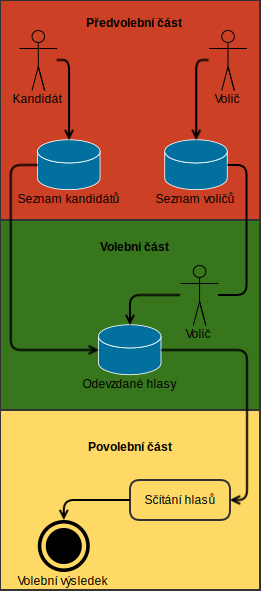
\includegraphics[scale=0.85]{obrazky/eml_konceptualni_pohled}

\caption{\label{fig:Konceptu=0000E1ln=0000ED-pohled-EML}Konceptuální pohled
na elektronické volby definovaný v EML\cite{EML}}
\end{figure}


\section{\label{sec:Druhy-elektronick=0000FDch-voleb}Typy elektronických
voleb}

Rozlišujeme různé typy elektronických voleb, a to podle fyzického
přístupu k zařízením. Zahraniční zdroje uvádějí rozdělení na i-voting
(internet voting) a e-voting (electronic voting).\cite{britannica_electronic_voting}

Mezi základní charakteristiku i-votingu patří to, že voliči odevzdávají
své hlasy z libovolného zařízení prostřednictvím internetu. V případě
i-votingu není volič nucen dostavit se do volební místnosti. Nevýhody
tohoto řešení spočívají v kompromitování voličova zařízení nebo znemožnění
volby různými útoky na technologickou infrastrukturu jakými jsou například
Denial of Service.

E-voting je takový typ elektronických voleb, při kterém se používají
speciální zařízení určená pouze pro průběh voleb. Mezi takovéto zařízení
patří DRE a skenovací stroje.

Pro skenovací stroje je charakteristické, že voličovo rozhodnutí je
skenováno z předem vyplněného hlasovacího lístku a následně uloženo
do paměti stroje. Jedná se tedy o decentralizovaný systém ukládání
dat. Takovéto zařízení bychom mohli přirovnat k volební urně použité
v klasických volbách.

DRE jsou zařízení umožňující voliči zaznamenat hlas prostřednictvím
obrazovky, kdy tento hlas je následně v zařízení zaznamenán. Principem
fungování se neliší od skenovacích strojů, mají však výhodu, že volič
může takovéto zařízení používat interaktivně. 

Je tedy patrno, že elektronické volby formou e-votingu se v principu
neliší od voleb klasických. Jejich výhodou je usnadnění sčítání hlasů.

Tuto typologii elektronických voleb nepovažuji za dobře zvolenou,
dávám přednost pojetí Petra Šindeláře, který rozděluje elektronické
volby dle jejich způsobu provedení, v závislosti na místu vykonání
aktu samotné volby, kdy místo vykonání volby je\cite{sindelar_elektronicke_volby}:
\begin{itemize}
\item kontrolovaný prostor
\item nekontrolovaný prostor
\end{itemize}

\section{Elektronické volby v kontrolovaném prostoru}

Elektronické volby v kontrolovaném prostředí označované též ,,poll-site
electronic voting`` jsou takové volby, které jsou provedené v přesně
definovaném čase prostřednictvím elektronického zařízení, definovaného
zákonem, které je umístěno v místě stanoveném zákonem (volební místnosti).
\cite{sindelar_elektronicke_volby}

Tento typ elektronického hlasování se dá také nazvat elektronickým
hlasováním na místě. Totožnost a oprávněnost voliče je ověřována fyzicky
na místě ve volební místnosti. Pro volbu, tedy udělení hlasu, je používáno
elektronické zařízení. Z definice neplyne, je-li hlas zpracován a
započten ihned transakčně nebo dávkově až po ukončení voleb, zároveň
není definováno, zda-li je hlas zaznamenán v lokálním úložišti hlasovacího
zařízení, či je přenesen některým komunikačním kanálem do centrálního
úložiště.

Mezi hlavní výhody tohoto typu voleb patří jeho důvěryhodnost v očích
voličů, vzhledem k jeho podobnosti ke klasickým volbám. Odpadá zde
nutnost elektronického ověření voliče a jeho ověření volební komisí
můžeme považovat za více než bezpečné. Zároveň u tohoto systému není
potřeba řešit anonymizaci hlasů pomocí kryptografie. Největším přínosem
je snížení náročnosti sčítání hlasů, z čehož plyne urychlení oznámení
výsledku voleb.

Vzhledem k tomu, že se tento typ voleb liší velice málo proti klasickým
volbám, autor považuje za jeho nevýhodu podobné náklady, které mohou
být i vyšší v případě varianty s centrálním úložistěm, neboť je nutné
zajistit i datový komunikační kanál pro přenos hlasů. Další možným
rizikem je možnost kompromitace hlasovacího zařízení škodlivým kódem.

\section{Elektronické volby v nekontrolovaném prostoru}

Za elektronické volby v nekontrolovaném prostoru považujeme takové
volby, které jsou provedené v přesně definovaném čase prostřednictvím
libovolného elektronického zařízení, splňujícího pouze technické požadavky
kompatibility se zvoleným volebním systémem, umístěným v libovolném
místě planety s nutnou dostupností komunikačního prostředí.\cite{sindelar_elektronicke_volby}

Takovýto typ elektronických voleb není závislý na fyzickém místě při
provedení samotného aktu volby. Z toho vyplívá největší výhoda tohoto
typu, protože zvyšuje komfort pro voliče, a to zejména z časových
důvodů. Volič může volit v jakýkoliv čas a z jakéhokoliv místa. V
dloudobém časovém horizontu je při tomto typu elektronických voleb
snížení nákladů, protože takový systém elektronických voleb je možné
využít při jejich dalším opakování.

Mezi hlavní nevýhody můžeme zařadit procesní a technickou náročnost
realizace takovýchto elektronických voleb. Z pohledu pořadatele voleb
je nutné zajistit identifikaci voliče a jeho oprávnění volit v jednotlivých
volbách. Dále je nutné zajistit anonymizaci hlasů. Další nevýhodou
pro realizaci elektronických voleb je také nízká přispůsobilost voličů
a tendence lpění na již zavedeném konceptu.

U elektronických voleb se setkáváme také s rizikem, že budou porušeny
principy tajnosti, důvěryhodnosti, svobody a všeobecnosti. Abychom
předešli porušení principu tajnosti, je potřeba propracovat bezpečný
systém šifrování hlasů. Autor práce se bude více této problematice
věnovat v kapitole \ref{chap:Implementace-elektronick=0000FDch-vole}.
Voliči mají bohužel většinou problém důvěřovat inovátorským postupům.
Právě toto spatřuje autor práce jako další riziko, kterému budou muset
implementátoři čelit. 

V neposlední řadě je potřeba zmínit také jako protiargument porušení
svobodné volby. Při realizaci elektronických voleb bude opravdu obtížné
zamezit porušení právě principu svobody. Avšak autor nalezl možné
řešení i na tento problém, které rozebere níže. Také bychom měli vzít
v úvahu princip všeobecnosti, který umožňuje voliči se zúčastnit voleb
jak aktivně, tak pasivně. Volič může namítat, že tento princip není
dodržen, jelikož nedisponuje dostatečným technickým zázemím a že stát
ho nemůže nutit vynaložit ne zrovna nízké náklady na jeho zabezpečení.
V tomto případě je však nasnadě jednoduché řešení, a to poskytnutí
potřebného zařízení například v místech státních úřadů.

\section{\label{sec:Porovn=0000E1n=0000ED-r=00016Fzn=0000FDch-typ=00016F}Porovnání
různých typů elekronických voleb}

V této části autor porovnává výhody a nevýhody výše zmíněných řešení
elektronických voleb. K tomuto porovnání je využita vicekriteriální
analýza, ve které jsou jednotlivým faktorům přiřazená diskrétní čísla
v oboru hodnot od jedné do deseti. Hodnota deset zde znázorňuje nejvyšší
možný užitek daného řešení. Tato analýza je zobrazena v tabulce \ref{tab:Porovn=0000E1n=0000ED-r=00016Fzn=0000FDch-typ=00016F}.

Mezi zvolené způsoby voleb autor zahrnuje elektronické volby v kontrolovaném
prostoru při použití DRE zařízení, elektronické volby v kontrolovaném
prostoru při použití optických skenerů a elektronické volby v nekontrolovaném
prostoru při použití internetových technologií. Mezi porovnávané faktory
patří:
\begin{itemize}
\item Zvýšení rychlosti sečtení hlasů – Snížení doby sečtění hlasů díky
využití informačních technologií, při kterých odpadá namáhavé a časově
náročné ruční sčítání hlasů.
\item Zvýšení pohodlnosti volby – Usnadňuje voličům provedení aktu volby,
ve smyslu snížení možnosti vložení neplatného hlasu, a zároveň umožňuje
voličům volit v jejich známém prostředí.
\item Snížení dlouhodobých nákladů – Snižování nákladů spojených s realizací
voleb v důsledku nižších nároků na fyzické zdroje. Snížení nákladů
je o to větší, čím častěji jsou volby uskutečňovány.
\item Tajnost volby – Nároky na zabezpečení utajení volby ve smyslu zaručení
anonymity volby voliče, jako jednoho z hlavních principů individuální
volby voliče.
\item Transparentnost volby – Složitost a potřeba odbornosti pro pochopení
vnitřního mechanismu celého procesu.
\item Přístupnost pro handicapované – Možnost zúčastnit se voleb pro handicapované
jedince bez nutnosti asistence, a tím i možná zvýšení účasti handicapovaných
voličů v jednotlivých volbách.
\item Pochopení volebního mechanismu laickou veřejností – Potřeba porozumění
voliče postupu volebního mechanismu při udělení hlasu a ochota voliče
naučit se a využít jiný posstup při hlasování. 
\item Riziko manipulace volebních výsledků – Faktor určující riziko podvodu
či nepřesnosti při sčítání nebo jiném zacházení s volebními hlasy.
Při elektronických volbách je nebezpečím kompromitace technických
zařízení náhodným či cizím a úmyslným zaviněním.
\end{itemize}
\begin{table}[H]
\begin{tabular}{|>{\centering}p{0.2\textwidth}||>{\centering}p{0.2\textwidth}|>{\centering}p{0.2\textwidth}|>{\centering}p{0.2\textwidth}|}
\hline 
 & Elektronické volby v kontrolovaném prostoru při použití optických
skenerů & Elektronické volby v kontrolovaném prostoru při použití DRE zařízení & Elektronické volby v nekontrolovaném prostoru při použití internetových
technologií\tabularnewline
\hline 
\hline 
Zvýšení rychlosti sečtení hlasů & 3 & 6 & 9\tabularnewline
\hline 
Zvýšení pohodlnosti volby & 1 & 4 & 7\tabularnewline
\hline 
Snížení dlouhodobých nákladů & 2 & 3 & 8\tabularnewline
\hline 
Tajnost volby & 6 & 5 & 2\tabularnewline
\hline 
Transparentnost volby & 9 & 6 & 2\tabularnewline
\hline 
Přístupnost pro handicapované & 1 & 5 & 8\tabularnewline
\hline 
Pochopení volebního mechanismu laickou veřejností & 9 & 8 & 5\tabularnewline
\hline 
Riziko manipulace volebních výsledků & 9 & 7 & 4\tabularnewline
\hline 
\end{tabular}

\caption{\label{tab:Porovn=0000E1n=0000ED-r=00016Fzn=0000FDch-typ=00016F}Porovnání
různých typů elektronických voleb}
\end{table}


\section{Technologie používaná v elektronických volbách}

V této části kapitoly se autor zabývá informačními technologiemi a
principy informačních technologií používaných v implementacích elektronických
voleb.

\subsection{\label{subsec:Asymetrick=0000E1-kryptografie}Asymetrická kryptografie}

Asymetrická kryptografie (označovaná někdy jako asymetrické šifrování)
je založena na principu vlastností matematických funkcí, které lze
vypočítat pouze v jednom směru. To znamená, že máme-li definovanou
funkci $y=f(x)$, kdy při jejím použití lze jednoduchým výpočtem získat
ze vstupní hodnoty $x$ výstupní hodnotu $y$, což znamená že takováto
funkce je řešitelná v reálném čase. Aby mohla být tato funkce využita
pro asymetrickou kryptografii je nutné zvolit takovou funkci, jejíž
inverzní funkce $f^{-1}$ je v reálném čase neřešitelná. \cite[str. 51]{aplikovana_kryptografie}

V asymetrické kryptografii je pro šifrování použit princip dvou klíčů,
kdy jeden je určen vždy pro zašifrování zprávy a druhým klíčem je
možné zprávu pouze dešifrovat. Jedná se o tyto klíče:
\begin{itemize}
\item Veřejný klíč – Jehož hodnota je veřejně známa.
\item Privátní klíč – Hodnota privátního klíče je známa pouze majiteli klíče
či vydávající entitě.
\end{itemize}
Veřejný klíč se používá pro zašifrování zprávy a privátní pro dešifrování
zprávy. Pokud chce uživatel komunikovat pomocí šifrovaného přenosu,
musí vygenerovat privátní a veřejný klíč. Veřejný klíč poskytne ostatním
uživatelům, kteří na jeho základě šifrují zprávu. Takovouto zprávu
mohou poslat nezabezpečeným kanálem, neboť její dešifrování je možné
pouze pomocí privátního klíče, který vlastní pouze uživatel, jenž
je příjemcem zprávy.\cite[str. 52]{aplikovana_kryptografie} 

Existuje mnoho způsobů a metod asymetrického šifrování, jejich společná
charakteristika je, že jsou založeny na jednocestných funkcích. Mezi
takové funkce řadíme například funkce řešící problém faktorizace čísla
nebo výpočet diskrétního logaritmu. (Používá Deffie-Hellman systém).
Existují i další funkce používané v asymetrické kryptografii, nicméně
v praxi jsou nejpoužívanější tyto zmíněné.\cite[str. 110]{aplikovana_kryptografie}

Nejčastěji je v asymetrické kryptografii užíván systém RSA. Jeho název
pochází z prvních písmen jmen tvůrců systému (Rivest, Shamir, Adelman).
RSA používá v jednosměrné funkci $f$ součin dvou velkých po sobě
následujících prvočísel (úloha typu P). Abychom v inverzní funkci
nalezli tento součin je nutné nalézt výstupní hodnotu inverzní funkce
$f$$^{-1}$, což je v tomto případě faktorizace výstupní hodnoty
funkce $f$ (úloha typu NP).

\subsection{\label{subsec:Digit=0000E1ln=0000ED-podpis}Digitální podpis}

Digitální podpis (Digital Signature) je systém autentizace pro ověřování
pravosti dat. Využívá principů asymetrické kryptografie, ale v inverzním
smyslu. Při digitálním podepisování uživatel podepisuje data svým
soukromým klíčem a za pomocí veřejného klíče se ověřuje autentičnost
těchto dat.\cite[str. 52]{aplikovana_kryptografie}

Autentičnost je ověřena takovým způsobem, že odesílatel dat k nim
přiloží a zašifruje zprávu (svůj podpis) svým soukromým klíčem. Tuto
přiloženou zprávu zveřejní a příjemce jí pomocí veřejného klíče dešifruje.
Pokud je zveřejněná zpráva totožná s dešifrovanou, pak je možné potvrdit
autentičnost odeslaných dat.

\subsection{\label{subsec:Hash}Hash}

Hash, označován také jako otisk nebo kontrolní součet, je výstupní
hodnota $y$ z použití jednosměrné funkce $y=f(x)$. Tato funkce je
charakterizována následujícími vlastnostmi\cite[str. 54]{aplikovana_kryptografie}:
\begin{itemize}
\item Různé vstupy $x$ funkce $f(x)$ mohou mít libovolnou délku, zároveň
výstupní hodnota $y$ funkce $f(x)$ musí nabývat konstantní délky.
\item Výstupní hodnota $y$ funkce $f(x)$ musí být vždy unikátní, nesmí
tedy nastat kolize. To znamená, že pro různé vstupní hodnoty $x$
nemůže nastat shodnost výstupních hodnot $y$.
\end{itemize}
Nejčastější případ použití hashů je při porovnávání dat a ověřování
jejich autentičnosti, kdy je nežádoucí, aby byla známa znalost těchto
dat při jejich porovnání. Při ověřování autentičnosti jsou vždy porovnávány
hodnoty hashů, tedy máme-li data $x$ a $x'$ a jejich hashe $h=f(x)$
a $h^{'}=f(x^{'})$, pak pro autentičnost těchto dat musí platit vztah
$h=h^{'}$

\section{Realizované elektronické volby}

V této části práce se autor pokusí seznámit čtenáře s již realizovanými
řešeními elektronických voleb.

\subsection{\label{subsec:Estonsko}Estonsko}

Estonská republika byla prvním státem jež realizovala elektronické
volby nekontrolovaném prostoru v celostátním rozsahu. V Estonsku probíhají
elektronické volby zároveň s klasickými, a to z důvodů obav estonských
vlád, že by mohli být elektronické volby kompromitovány. Proto elektronické
volby z časového hlediska probíhají před klasickými volbami. Zároveň
volič může v klasických volbách změnit své rozhodnutí, při kterém
udělil hlas ve volbách elektronických.

Elektronické volby v Estonsku vycházejí z principu, že musí být co
nejvíce podobné klasickým volbám a jejich zabezpečení nesmí být o
nic menší než-li u klasických voleb. \cite{riigikogu_election_act}

Dle legislativy Estonské republiky probíhají elektronické volby od
šestého do čtvrtého dne od vyhlášení voleb a musí splňovat tyto požadavky
\cite{riigikogu_election_act,e_voting_estonsko}:
\begin{itemize}
\item Ve dnech, kdy probíhají elektronické volby, mohou voliči volit na
webových stránkách Národní Volební Komise.
\item Volič se identifikuje na základě digitálního certifikátu, který je
vložený v jeho průkazu totožnosti.
\item Po identifikaci voliče, je zobrazen ve webové stránce konsolidovaný
seznam kandidátů v jeho volebním okrsku, dle trvalého pobytu voliče.
\item Volič si na webové stránce může vybrat svého preferovaného kandidáta
z jemu zobrazeného konsolidovaného seznamu kandidátů. Zároveň volič
podepíše svoji volbu svým digitálním certifikátem
\item Po výběru kandidáta je voliči na webové stránce zobrazeno ohlášení,
že systém elektronických voleb započítal jeho hlas.
\item Volič může změnit své rozhodnutí ve volbě do čtvrtého dne před sečtením
hlasů, a to jak pomocí elektronického volebního systému nebo klasickým
provedením volby ve volební místnosti. V případě změny voličova rozhodnutí,
je jeho předchozí hlas ze systému odstraněn. V případě, že volič provede
akt volby klasickým způsobem, nebere se na jeho hlas provedený pomocí
systému elektronických voleb zřetel.
\end{itemize}
Estonské elektronické volby jsou z konceptuálního hlediska velice
podobné korespondenčnímu hlasování\footnote{Korespondenční hlasování, někdy označované jako hlasování ,,per rollam``,
není při volbách v ČR používáno, První výskyt tohoto pojmu v české
legislativě se uskutečnil v době nabytí platnosti zákonu o obchodních
korporacích.\cite{zakon_o_obchodnich_korporacich}}, které je využito v případě, pokud volič volí v jiné volební místnosti,
než ve volební místnosti mu určené na základě jeho trvalého pobytu.
Část volebního procesu je pomocí korespondenční metody definována
takto \cite{e_voting_estonsko} :
\begin{enumerate}
\item Volič se identifikuje volební komisi.
\item Volič zvolí preferovaného kandidáta na volebním lístku a ten následně
vloží do obálky.
\item Tuto obálku vloží do další vnější obálky, na kterou volební komise
napíše informace o voličovi.
\item Vnější obálka je před sčítáním dopravena do volební místnosti, ve
které by volič volil za standardních okolností a je volební komisí
otevřena. Poté volební komise hodí vnitřní obálku do volební urny.
\end{enumerate}
\begin{figure}
\includegraphics{obrazky/korespondencni_hlasovani_estonstko}

\caption{\label{fig:Zn=0000E1zorn=00011Bn=0000ED-elektronick=0000FDch-voleb-pomoc=0000ED-koresponden=00010Dn=0000EDho-hlasov=0000E1n=0000ED}Znázornění
elektronických voleb pomocí korespondenčního hlasování\cite{e_voting_estonsko}}
\end{figure}

Na rozdíl od použití papírových obálek v korespondenčním hlasování
používá systém elektronických voleb vlastností asymetrické kryptografie.
Viz \ref{subsec:Asymetrick=0000E1-kryptografie}. Volič podepíše svůj
hlas veřejným klíčem elektronického volebního systému a výsledná data
opět podepíše, ale svým privátním klíčem. Podobnost s korespondenčním
hlasováním ilustruje obrázek \ref{fig:Zn=0000E1zorn=00011Bn=0000ED-elektronick=0000FDch-voleb-pomoc=0000ED-koresponden=00010Dn=0000EDho-hlasov=0000E1n=0000ED}.
Hlasy jsou v systému elektronických voleb setříděny, odebrány neplatné
hlasy, kdy za platný hlas je voličovo rozhodnutí, které je na časové
ose nejblíže k času ukončení voleb a zahájení sčítání hlasů. Z vnějších
obálek je sestaven seznam voličů, jež hlasovali pomocí systému elektronických
voleb, a poté jsou otevřeny. Obsah otevřených vnějších obálek, tedy
vnitřní obálka, je přeposlána části systému, určenému pro sčítání
hlasů, která obsahuje privátní klíč elektronického volebního systému.
Tato část dešifruje obsah obálek a sečte hlasy kandidátů udělené pomocí
elektronických voleb.\cite{e_voting_estonsko}

V estonském systému elektronických voleb je tajnost volby zachována
způsobem, že žádná část systému nemá ve stejný čas přístup k privátnímu
klíči systému a privátnímu klíči voliče. \cite{e_voting_estonsko}

\subsubsection{Architektura systému}

Architektura systému elektronických voleb v Estonsku se skládá ze
čtyř vzájemně propojených částí, jejich vazby jsou znázorněny na obrázku
\ref{fig:Architektura-elektronick=0000FDch-voleb-estonsko}. Jedná
se o tyto části:

\begin{figure}
\includegraphics{obrazky/achitektura_e_volebniho_systemu_estonsko}

\caption{\label{fig:Architektura-elektronick=0000FDch-voleb-estonsko}Architektura
elektronických voleb v Estonsku\cite{e_voting_estonsko}}
\end{figure}

\begin{itemize}
\item Rozhraní pro voliče – Toto rozhraní je implementováno pomocí webové
aplikace. Z technologického hlediska se jedná o ActiveX applet podepsaný
Národní Volební Komisí, který je nahrán do WWW prohlížeče voliče a
umožňuje voliči zašifrovat a podepsat svůj hlas.
\item Centrální systém – Přijímá data z výše zmíněné volební aplikace, která
následně zpracovává. Výstupem této části jsou spočítané hlasy kandidátů.
Tento systém se skládá ze tří částí.

\begin{itemize}
\item Vote Forwarding Server (VFS) – Z technologického principu se jedná
a autentizační proxy server, který ověří identitu voliče a podepsanou
obálku s daty přepošle na Vote Storage Server. Při ověřování identity
se VFS dotazuje do databází voličů a kandidátů. 
\item Vote Storage Server (VSS) – Přijímá data z Vote Forwarding Serveru
a ukládá je. Po ukončení hlasování jsou v této databázi zpracována
data dávkově. Nejprve jsou data očištěna. Pod očištěním dat autor
práce rozumí odstranění neplatných hlasů voličů, kteří opakovali volbu
jak elektronicky, tak klasickým způsobem. Následně jsou dávkovou procedurou
otevřeny vnější obálky a připravena data pro přenesení do Vote Counting
Application.
\item Vote Counting Application (VCA) – Tato část jako svůj vstup přijímá
očištěná data z Vote Storage Serveru a privátní klíč systému. Na základě
tohoto vstupu dešifruje hlasy voličů, sečte je a vygeneruje sestavu
dat pro interpretaci volebního výsledku. 
\end{itemize}
\item Správa klíčů – Jedná se o způsob zacházení se šifrovacími klíči v
elektronickém volebním systému.
\item Audit – Systém kontroly řádného průběhu elektronických voleb.
\end{itemize}
Pro zlepšení zabezpečení tohoto systému je jediná komponenta přístupná
ze sítě Internet Vote Forwarding Server. Zbytek technologické části
systému je v demilitarizované zóně\footnote{Demilitarizovaná zóna je prostředek, používaný pro zabezpečení v počítačových
sítích, ve kterém je možné komunikovat s vnějšími sítěmi pouze skrze
jeden předem vybraný uzel sítě.}. Vzhledem k tomu, že obsahy vnitřních obálek s hlasy voličů jsou
velice důvěrná data, je bezpečnost zvýšena tím, že datový přenos mezi
Vote Storage Serverem a Vote Counting Application není realizován
pomocí počítačových sítí, ale data jsou přenášena fyzickým datovým
nosičem\footnote{Pod pojmem fyzický datový nosič si můžeme představit taková média
jakými jsou například CD, DVD, či magnetické pásky.}.

\subsubsection{Průběh volebního procesu při použití elektronického volebního systému}

Fyzický akt volby je realizován interakcí voliče a rozhraním elektronického
volebního systému ve formě klientské www aplikace, serverová část
aplikace je provozována na Vote Forwarding Serveru.
\begin{enumerate}
\item Volič se identifikuje Vote Forwarding serveru na základě své identifikační
karty a dle jeho PIC\footnote{Personal identification Code (Osobní identifikační kód občana) je
v Estonské republice identifikační číslo občana, jeho ekvivalentem
v České republice je buď rodné číslo nebo číslo občanského průkazu} je vyhledán v příslušném seznamu voličů a VFS předá klientské části
aplikace seznam kandidátů ve voličově obvodu. V případě, že volič
již jednou volil, je v tomto kroku o jeho předchozí volbě informován.
\item Volič v klientské aplikaci vybere svého preferovaného kandidáta a
je klientskou částí aplikace vyzván k potvrzení svého rozhodnutí.
\item Po potvrzení voličova rozhodnutí je klientskou části aplikace zašifrován
jeho hlas za pomocí veřejného klíče elektronického volebního systému,
zároveň volič tento hlas podepíše svým klíčem uloženým v identifikační
kartě a vytvoří tak pomyslnou vnější obálku popisovanou výše.
\item Jeho hlas je předán z VFS do VSS, kde je zároveň uložena časová značka
provedení volby voličem. Po ukončení této transakce je kaskádově v
systému vyslána zpráva zpět voliči, že jeho hlas byl zaznamenán. Na
konci tohoto kroku je ukončena veškerá komunikace s klientskou částí
aplikace.
\end{enumerate}
Tento proces může volič opakovat neustále do času, kdy je ukončeno
hlasování. Ze všech kroků tohoto procesu jsou generovány logy komponent
elektronického volebního systému pro jeho audit viz tabulka \ref{tab:Syst=0000E9m-log=00016F}.

\subsubsection{Správa klíčů}

Z hlediska zabezpečení elektronického volebního systému je správa
klíčů tím nejrizikovějším místem v systému. Pro každé volby je vygenerován
pár klíčů (privátní a veřejný klíč) pro asymetrické šifrování. Privátní
klíč se používá pro dešifrování hlasů ve Vote Counting Application
a veřejný klíč ve webové aplikaci pro voliče. Z hlediska napadení
elektronického volebního systému v šifrování hlasů jsou v Estonském
řešení vyskytují dvě možné hrozby:
\begin{itemize}
\item Zkompromitování či zveřejnění privátního klíče systému – Kompromitace
principu tajnosti hlasování a možnost zveřejnění hlasů voličů.
\item Ztráta nebo porušení integrity privátního klíče systému – Nemožnost
dešifrovat výsledky voleb Národní Volební Komisí, a tím je celé zneplatnit.
\end{itemize}
Aby se předešlo zneužití klíčů v elektronických volbách jsou oba klíče
generovány HSM (Hardware Security Module) zařízením\footnote{HSM je zařízení pro generování a správu klíčů, generování klíče v
těchto zařízeních je již implementováno v hardwaru zařízení. HSM zařízení
se vyskytují ve formě přídavných karet do počítačů nebo čistě externí
s možností přímého propojení s počítačem.}, a to takovým způsobem, že obsah privátního klíče nikdy toto zařízení
neopustí. Pro provádění operací s HSM zařízením je vyžadována přítomnost
čtyř členů ze sedmičlenné Národní Volební Komise, všechny operace
s HSM zařízením jsou pečlivě dokumentovány, archivovány a podrobeny
auditům.\cite{e_voting_estonsko} Po zákonné lhůtě pro podání žaloby
pro neregulérnost voleb a v případě, že takováta žaloba nebyla podána,
je privátní klíč vždy zničen.

\subsubsection{Audit elektronických voleb}

Audit elektronických voleb spočívá v kontrole integrity dat, z různých
částí systému, aby byl zachován princip tajnosti voleb je u dat týkající
se hlasů voliče používán hash (viz. \ref{subsec:Hash}) těchto dat.
Pro umožnění auditu voleb systém generuje několik logů, z každé jeho
části. Obsah logů a jejich význam ilustruje tabulka \ref{tab:Syst=0000E9m-log=00016F}.

\begin{table}
\begin{tabular}{|c|>{\raggedright}p{0.2\textwidth}|c|c|}
\hline 
Název logu & Obsah logu & Význam logu & komponenta systému generující log\tabularnewline
\hline 
\hline 
LOG1 & PIC, hash hlasu & přijaté hlasy & Vote Forwarding Server\tabularnewline
\hline 
LOG2 & PIC, hash hlasu,\linebreak důvod zneplatnění & zneplatněné hlasy & Vote Storage Server\tabularnewline
\hline 
LOG3 & PIC, hash hlasu & hlasy k sečtení & Vote Storage Server\tabularnewline
\hline 
LOG4 & hash hlasu & neplatné hlasy & Vote Counting Application\tabularnewline
\hline 
LOG6 & hash hlasu & sečtené hlasy & Vote Counting Application\tabularnewline
\hline 
\end{tabular}

\caption{\label{tab:Syst=0000E9m-log=00016F}Systém logů při provádění auditu
voleb\cite{e_voting_estonsko}}

\end{table}


\subsubsection{Zhodnocení realizace elektronických voleb v Estonsku}

Vzhledem k tomu, že estonský systém elektronických voleb vychází z
korespondenčního hlasování, které je ověřené desetiletími praktického
užívání v mnoha evropských státech, považuje jej autor jako velice
zdařilý způsob realizace elektronických voleb. Jako mimořádnou výhodu
vidí autor v možnosti opakování volby voliče, která v této realizaci
řeší zachování principu svobodné volby. Za hlavní nevýhodu považuji
způsob implementace tohoto elektronického volebního systému, neboť
byla vyvíjena soukromým sektorem jako individuální aplikační software\footnote{Individuální aplikační Software (IASW) je takový software, který je
vytvořen přímo na míru řešeného problému, zároveň je navržen tak,
aby optimálně podporoval proces při řešení problému.\cite[str. 59]{Vorisek_rizeni_podnikove_informatiky}} pro potřeby realizování elektronických voleb do parlamentu Estonské
republiky. U voleb na národní úrovni, ze kterých vzejde reprezentace
legislativní složky moci státu, by implementace jejich elektronické
varianty měla být určitě licencována s podmínkou otevřenosti zdrojového
kódu.

\subsection{Švýcarsko}

Švýcarská konfederace je státem, ve kterém je uplatňována tzv. polopřímá
demokracie\footnote{Mezi polopřímé demokratické systémy zařazujeme takové systémy, které
fungují na principech zastupitelské demokracie, avšak je v nich hojně
využíváno prvků přímé demokracie, převážně referend a lidových iniciativ.\cite[str. 16]{poloprima_demokracie_ve_svyrarsku}}. Volby probíhají ve třech úrovních Švýcarské konfederace, přičemž
mezi nimi platí absolutní princip subsidiarity\footnote{Princip subsidiarity je politickou zásadou, že veškeré rozhodování
a odpovědnost se odehrává na nejnižším stupni veřejné správy. Absolutní
princip subsidiarity je ve Švýcarské konfederaci založen na systému
propůjčení státní moci od nejnižšího správního celku vždy k vyššímu.\cite[str 35]{poloprima_demokracie_ve_svyrarsku}}.\cite[str. 34]{poloprima_demokracie_ve_svyrarsku} Tyto úrovně jsou:
federální, kantonální a komunální. Vzhledem k velkému počtu voličského
rozhodování je Švýcarská konfederace jedním z prvních států, který
si osvojil metodu korespondenčního hlasování (viz. \ref{subsec:Estonsko}).

Elektronické volby ve Švýcarsku jsou na základě legislativy povoleny
od roku 2002, a to pouze v kantonální a komunální úrovni. Na základě
decentralizovaného charakteru státní moci Švýcarské konfederace je
způsob technického řešení elektronických voleb přenechán odpovědnosti
jednotlivých kantonům.\cite{federal_act_on_political_rights} Dle
Švýcarské legislativy musí systém elektronických voleb splňovat bezpečnost
a spolehlivost, jako systém korespondenčního hlasování. Systém elektronických
voleb musí splňovat tyto požadavky\cite{federal_ordinance_on_political_rights}:
\begin{itemize}
\item Voleb se mohou zúčastnit pouze oprávnění voliči.
\item Každý volič má pouze jeden hlas a může ho uplatnit pouze jednou.
\item Každý udělený hlas musí být započítán.
\item Nemožnost zásahu třetí strany do volebního rozhodování voliče.
\item Nemožnost zisku znalosti o obsahu udělených hlasů třetí stranou.
\item Nemožnost systémového volebního podvodu.
\end{itemize}
Elektronické volby v nekontrolovaném prostoru začali zavádět kantony
Ženeva, Neuchatel a Curych.\cite{three_case_studies_from_switzerland}
Autor se zaměří především na popis elektronického volebního systému
v kantonu Ženeva, protože Ženevská státní moc nabídla jejich systém
i ostatním kantonům, kde se také zavádí.\cite{three_case_studies_from_switzerland}

V roce 2001 spustila vláda kantonu Ženeva projekt zavedení elektronického
volebního systému v nekontrolovaném prostoru. Již v roce 2002 se začal
systém zkoušet na vzorku 16000 vysokoškolských studentů, avšak jeho
použití bylo schváleno v kantonálním referendu v roce 2009. Pro možnost
hlasovat elektronicky se vyslovilo 70,2\% voličů. V roce 2011 proběhly
první komunální a kantonální volby, ve kterých byla možnost použít
elektronický volební systém.\cite{the_geneva_internet_voting_system}

Ženeva do svého elektronického volebního systému zahrnula následující
požadavky\cite{the_geneva_internet_voting_system}:
\begin{itemize}
\item Elektronický volební systému musí být oddělený od ostatních kantonálních
informačních systémů.
\item Vhozené hlasy musí být zpracovávány v systému v jiném pořadí, než
ve kterém byly uděleny.
\item Dohled a zajištění bezpečnosti elektronického volebního systému a
jeho dat je prováděna nezávislou volební komisí. Tato komise se skládá
ze zástupců volebních stran a vybraných IT specialistů.
\item Nezávislá volební komise si může vyžádat jakékoliv dokumenty týkající
se elektronického volebního systému. Zároveň může nařídit jakýkoliv
audit, zkoušku či studii jí delegovanými specialisty
\item Volební komise a místní akademická obec mají právo nahlížet kdykoliv
do zdrojových kódů elektronického volebního systému.
\item Elektronický volební systém je v pravidelných intervalech podrobován
auditu, obsah a výsledek auditu musí být dostupný veřejnosti.
\end{itemize}

\subsubsection{Architektura systému}

Architektura systému elektronických voleb v Ženevě se skládá z mnoha
vzájemně propojených částí, jejich vazby jsou znázorněny na obrázku
\ref{fig:Architektura-elektronick=0000FDch-voleb-v-Zeneve}. Jedná
se o tyto části\cite{the_geneva_internet_voting_system,uncovering_veil_on_geneva_voting_solution}:

\begin{figure}
\includegraphics{obrazky/achitektura_e_volebniho_systemu_svycarsko}

\caption{\label{fig:Architektura-elektronick=0000FDch-voleb-v-Zeneve}Architektura
elektronických voleb v Ženevě\cite{the_geneva_internet_voting_system}}

\end{figure}

\begin{itemize}
\item Rozhraní pro voliče – Toto rozhraní je implementováno pomocí webové
aplikace. Z technologického hlediska se jedná o podepsaný Java applet,
který je nahrán do WWW prohlížeče voliče a umožňuje voliči odevzdat
a podepsat svůj hlas. Následně je hlas odeslán pomocí šifrovaného
kanálu do volebního systému.
\item Volební systém – Přijímá data z výše zmíněné volební aplikace, která
následně zpracovává. Tento systém se skládá z několika částí. Operace
mezi částmi volebního systému probíhají atomicky v jedné transakci.
\begin{itemize}
\item Web server – Web server poskytuje aplikaci klientovi, nezpracovává
však žádná data odeslaná klientskou aplikaci, již zmíněným Java appletem.
Data zasílá jako obyčejný proxy server aplikačnímu serveru.
\item Aplikační server – Přijímá data z Web serveru, kdy se zaslaným hlasem
vytvoří jednu relaci a rozdělí data z klientské aplikace. Tato data
následně odešle do registru voličů a elektronické volební urny.
\item Registr voličů – Přijímá část dat z Aplikačního serveru. V tomto registru
se pouze ukládá záznam, že daný volič vhodil svůj hlasovací lístek.
\item Elektronická volební urna – Tato část elektronického volebního systému
ukládá data z elektronického hlasovacího lístku voliče.
\end{itemize}
\end{itemize}

\subsubsection{Příprava volebního procesu}

V přípravné fázi volebního procesu jsou do systému voleb naimportována
data z různých zdrojů, a to převážně z registru obyvatel, který spravuje
kantonální veřejná správa. Jedná se o tato data\cite{uncovering_veil_on_geneva_voting_solution}:
\begin{itemize}
\item Volební obec a okrsek
\item Data týkající se volby, tedy například návrh textu v referendu nebo
listina kandidátů
\item Data obsahující informaci o voliči, konkrétně jméno, příjmení a trvalé
bydliště voliče.
\item Data umožňující voliči hlasovat v elektronickém systému voleb. Mezi
tato data patří číslo volební karty, datum narození voliče, volební
okrsek voliče na základě jeho trvalého bydliště, heslo k systému elektronických
voleb a kontrolní součet.
\end{itemize}
Tato data nejsou agregována v žádné databázi, nýbrž jsou z nich přímo
vygenerovány tiskové soubory volebních karet voličů. Volební karta
je po svém vytisknutí a předání voliči používána jako jeho indentifikátor
a hlasovací lístek ve fyzické volební místnosti nebo při korespondenční
volbě. Zároveň údaje na volební kartě slouží k autentizování voliče
v elektronickém systému voleb.

Po distribuci volebních karet následuje zapečetění elektronické volební
urny. Z technického hlediska je urna zapečetěna na základě třech klíčů.
Jedná se o klíč pro symetrickou kryptografickou funkci a jeden pár
klíčů pro asymetrickou kryptografickou funkci.\cite{uncovering_veil_on_geneva_voting_solution}

Symetrická šifrovací funkce je v systému používána pro výpočet integrity
elektronické volební urny. Funkce pro zachování integrity je založena
na základě počtu vhozených hlasů, kdy s každým nově vhozeným hlasem
je hodnota počtu vhozených hlasů dešifrována, poté zvýšena o jedna
a následně opět zašifrována. 

Asymetrická kryptografie je v elektronické volební urně použita tak,
že veřejný klíč je uložen v systému a je použit pro zašifrování vkládaných
hlasů do volební urny. Soukromý klíč je použit při dešifrování vhozených
hlasů volební komisí a je bezpečně uložen na fyzickém datovém nosiči.

\subsubsection{Správa a zabezpečení klíčů}

Pro zabezpečení klíčů, tedy nejrizikovějšího místa elektronického
volebního systému je použit následující postup, kdy tok dat je znázorněn
na obrázku\cite{uncovering_veil_on_geneva_voting_solution}:

\begin{figure}
\includegraphics[width=0.8\textwidth]{obrazky/sprava_klicu_svycarsko}

\caption{\label{fig:Ilustrace-toku-dat-pri-sprave-klicu}Ilustrace toku dat
při správě klíčů\cite{uncovering_veil_on_geneva_voting_solution}}

\end{figure}

\begin{enumerate}
\item Administrátor elektronického volebního systému před členy volební
komise vygeneruje za použití kvantového generátoru náhodných čísel\footnote{Klasické generátory náhodných čísel, používají k získání entropie
elektromagnetický šum z okolí. Kvantový generátor náhodných čísel,
který je použit v ženevském systému elektronických voleb získává entropii
ze sekvencí fotonů denního světla.\cite{the_geneva_internet_voting_system}} symetrický klíč a jeden pár asymetrických klíčů. 
\item Následně je soukromý klíč zabezpečen dvěmi hesly pro nemožnost získání
jeho hodnoty. Tato hesla zadávají dvě skupiny členů volební komise.
Zároveň tato hesla zapíší na papír a vloží do obálky, která je předána
do úschovy kantonálnímu notáři.
\item Je vygenerována kolekce klíčů. Tato kolekce je poté uložena na dva
fyzické datové nosiče. Vždy se jedná o CD a přenosné USB médium.
\item Fyzické datové nosiče jsou dány do úschovy IT oddělení policie.
\item Symetrický klíč a veřejný asymetrický klíč jsou zabezpečenou cestou
nahrány do elektronického volebního systému.
\item Pro dešifrování hlasů je použit soukromý klíč, který se po ukončení
hlasování získá opačným postupem předchozích bodů.
\end{enumerate}

\subsubsection{Průběh volebního procesu při použití elektronického volebního systému}

Po připravení volebního procesu, mohou voliči interagovat s rozhraním
elektronického volebního systému. Volební proces z pohledu voliče
je velice jednoduchý, odevzdat v něm hlas je otázkou maximálně dvou
minut\cite{the_geneva_internet_voting_system,uncovering_veil_on_geneva_voting_solution}.
\begin{enumerate}
\item Volič si ve webovém prohlížeči načte rozhraní elektronického volebního
systému.
\item Volič se indetifikuje v rozhraní elektronického volebního systému
na základě jeho volební karty, tj. vyplní číslo volební karty, která
se skláda z šestnácti číslic a potrvdí podmínky užívání elektronického
volebního systému.
\item Následně volič v rozhraní volebního systému vybírá kandidáty z kandidátních
listin, či návrh textu v referendu.
\item V další obrazovce rozhraní, je voliči zobrazena jeho volba pro kontrolu
jeho rozhodnutí. Zároveň v této obrazovce je volič povinen vyplňit
do formuláře své heslo, datum narození a volební okrsek. Po vyplnění
formuláře volič stiskne tlačítko hlasovat a elektronický volební systém
jeho hlas započítá.
\end{enumerate}

\subsubsection{Zhodnocení realizace elektronických voleb ve Švýcarsku}

Švýcarský elektronický volební systém vychází v konceptuálním pojetí
ze systému korespondenčního hlasování. Za hlavní výhodu Švýcarského
řešení autor považuje to, že je pouze doplňkem korespondenční volby.
Pro funkčnost takovéhoto elektronického volebního systému není nutné,
aby orgány švýcarské veřejné správy modifikovaly identifikační doklady
občanů, neboť touto modifikací je například umístění specializovaného
čipu do dokladu. Pro funkční řešení stačilo do volební karty doplnit
data nutná pro použítí elektronického volebního systému. Z tohoto
důvodu se autor domnívá, že náklady na nasazení volebního systému
a jeho provoz jsou velice nízké, oproti jiným řešením. Ovšem nevýhodou
takovéto provázanosti je závislost elektronického hlasování na hlasování
korespondeční. Mezi další výhody švýcarského řešení je jeho legislativní
úprava, která umožňuje odborné veřejnosti provádět audit elektronických
voleb, a to i na úrovni zdrojového kódu.

\chapter{\label{chap:Anal=0000FDza-elektronick=0000FDch-voleb}Analýza elektronických
voleb Strany svobodných občanů}

\section{O straně svobodných občanů}

Strana svobodných občanů (zkráceně Svobodní, někdy nesprávně SSO)
je mladou politickou stranou, která vznikla na Ustanovujícím sněmu
14. února 2009 jako důsledek změn na pravicové politické scéně, a
to především odkloněním strany Občanských demokratů ke středu politického
spektra. Tato v této době vládní politická strana pokračovala v zadlužování
státu a nebránila se předávání pravomocí do Bruselu. 

Prvopočátkem vzniku Strany svobodných občanů byla nespokojenost některých
členů ODS s touto situací, kteří již v roce 2001 sepsali pro ideovou
konferenci ODS dokument nazvaný Manifest českého eurorealismu. Manifest
se sice nestal oficiálním programovým dokumentem strany, ale shrnul
postoje euroskeptického křídla ODS, které mimo jiné v dokumentu uvádí,
že při rozhodování mezi nadnárodním a mezivládním modelem evropské
integrace by se ČR měla jasně postavit za mezivládní. Dalším významným
podnětem pro vznik Svobodných byl 19. kongres ODS, kde bylo voleno
nové vedení strany, které neodmítlo ratifikaci Lisabonské smlouvy.

Obsah Lisabonské smlouvy byl vypracován v bilaterálních jednáních
během německého předsednictví v Radě Evropské unie, definitivně dohodnut
a schválen na zasedání Evropské rady v Bruselu v červnu 2007. Dle
Lisabonské smlouvy se již nepoužívá při hlasování v Radě systém trojí
většiny v (definované počtem států, jejich váženými hlasy a podílem
obyvatelstva, který na EU představují), ale zavádí se systém dvojí
většiny, resp. přestává se používat kritérium vážených hlasů. Pro
přijetí rozhodnutí se tak musí vyslovit 55 \% členských států, které
tvoří současně 65 \% obyvatel EU. Tímto způsobem hlasování mohou např.
jen čtyři velké země EU zablokovat rozhodnutí Rady. Mimo jiné Lisabonská
smlouva definuje mechanismy, které dávají EU možnost získávat nové
pravomoci a rušit právo veta v dalších oblastech bez další ratifikace.

I když uvedené události předcházely vzniku Strany svobodných občanů,
hlavním důvodem se dle vyjádření zakladatele a předsedy strany Petra
Macha stala chybějící liberální strana, která by hájila svobodu jednotlivce
a snažila se o liberalizaci prostředí. Svoboda jednotlivce, ale také
jeho zodpovědnost, je hlavní myšlenkou Svobodných.

Podíváme-li se na politický program a další materiály Svobodných ve
srovnání se znaky jiných ideologií, je možné konstatovat, že se prolíná
klasický liberalismus a liberální konzervatismus. To, že Svobodní
jsou na veřejnosti představováni hlavně jako strana euroskeptická,
vyplývá z jejich liberální ideologie, neboť EU pro ně přestavuje omezování
osobních svobod jednotlivce a následně i svobodu rozhodování suverénního
státu. Evropská unie dle Svobodných nenaplňuje ideály liberalismu,
naopak na ně útočí a ohrožuje tak podstatu demokracie. Řada zákonů
je v Poslanecké sněmovně schvalována tzv. v souladu se Směrnicemi
EU, resp. tyto zákony se schválit musí, a tudíž jsou v přímém rozporu
s demokratickými zásadami. Otázkou zůstává, proč současný Parlament
ČR neschválil možnost uskutečnění referenda o odchodu z EU, neboť
sice v roce 2003 se 77\% českých občanů se vyjádřilo pro vstup do
EU, avšak přijetím Lisabonské smlouvy a zahraniční politikou EU, danou
především představiteli Německa a Francie, se toho poměrně dost změnilo.

Podle období vzniku strany by se mohla jevit evropská problematika
jako stěžejní. Podíváme-li se ale na program Svobodných, zjistíme,
že evropská tématika není hlavním bodem programu, jak se jeví dle
představování Svobodných v našich hromadných sdělovacích prostředcích.
Program Svobodných zahrnuje nejen otázky zahraniční politiky a vnější
bezpečnosti státu, ale i hospodářství, daňové a měnové politiky, silniční
dopravy, ochrany životního prostředí, zdravotnictví, sociální politiky,
školství, vědy, zemědělství a veřejné správy a samosprávy. V celém
programu se prolínají základní postoje Svobodných, které je možné
stručně charakterizovat slovy: svoboda, odpovědnost, spravedlnost.
V základním programovém cíli strany je uvedeno, že se jedná o stranu
občanů, kteří chtějí žít ve svobodné a suverénní zemi, spravované
státem, jenž k nim i k jejich životu, majetku, svobodě a osobní odpovědnosti
chová úctu. Své cíle strana prosazuje na základě svobodné diskuse
demokratickými metodami při respektování platných právních předpisů. 

\subsection{Organizační struktura Svobodných}

Z organizačního hlediska je struktura Svobodných koncipována tak,
aby reflektovala dělbu státní moci České republiky . Orgány strany
mají vždy pouze zákonodárnou, výkonnou či soudní moc. Dle stanov Strany
svobodných občanů jsou zřízeny tyto orgány\cite{svobodni_stanovy}:
\begin{itemize}
\item Republikový sněm – Tento orgán je nejvyšším orgánem strany. Jedná
se o legislativní orgán. Každý člen Strany svobodných občanů je vždy
členem republikového sněmu. Všichni členové republikového sněmu mají
právo rozhodovat (hlasovací právo). V přirovnání ke státu se defacto
jedné o občany státu.
\item Republikový výbor – Jedná se o reprezentaci republikového sněmu v
době, kdy republikový sněm nezasedá. Republikový výbor je nepřímé
demokratické zastoupení republikového sněmu. Ve své podstatě je obdoba
parlamentu ve straně.
\item Republikové předsednictvo – Je statutárním a výkonným orgánem strany.
Předkládá republikovému výbory vlastní návrhy týkající se činnosti
strany.
\item Rozhodčí komise – Rozhoduje ve sporech mezi členy strany a odpovídá
za závazný výklad stanov.
\item Kontrolní komise – Dohlíží na hospodoření výkonných orgánů strany
a dodržování usnesení orgánů a stanov.
\item Volební komise – Organizuje a technicky zajišťuje připravenost konat
volby ve straně.
\item Krajská sdružení – Rozdělení republikového sněmu na uzemním principu.
\begin{itemize}
\item Krajský sněm – Legislativní orgán strany na krajské úrovni.
\item Krajské předsednictvo – Plní úkoly krajského sněmu a předkládá mu
vlastní návrhy týkající se činnosti strany na krajské úrovni.
\end{itemize}
\end{itemize}

\subsection{Informační systémy Svobodných}

Po vzniku strany v roce 2009 byl ve straně implementován a zaveden
informační systém \emph{Databáze členů. }Jednalo se o monolitický
systém postavený na webové aplikaci, který zajišťoval podporu pouze
dvou agend a to:
\begin{itemize}
\item evidování členů a příznivců
\item elektronické korespondenční hlasování
\end{itemize}
Podpora těchto agend byla z hlediska funkčnosti dosti omezená a míra
bezpečnosti informačního systému dosahovala velice nízké úrovně. Databáze
členů podporovala následující procesy:
\begin{enumerate}
\item Zaregistrování nového člena a příznivce
\item Spárování platby člena či příznivce
\item Poskytování informací o členech a příznivcích strany – Nebylo implementováno
dělení do organizačních struktur strany a k datovým strukturám nebylo
možné delegovat oprávnění k přístupu jednotlivými uživateli informačního
systému.
\item elektronické korespondenční hlasování – Nesplňovalo bezpečnostní požadavky
elektronických voleb viz část \ref{sec:Porovn=0000E1n=0000ED-r=00016Fzn=0000FDch-typ=00016F}.
Z technologického hlediska nebyla použita žádná kryptografická metoda
při zaznamenávání vložených hlasů. Hlas v elektronickém korespondenčním
hlasování byl zaznamenáno pouze jako hash voličova rozhodnutí.
\end{enumerate}
Z tohoto důvodu se v roce 2014 republikový sněm usnesl na potřebu
použítí nového informačního systému. Požadavky na něj jsou následujcí:

Z tohoto důvodu byl vyvinut a nasazen nový informační systém, 

\subsection{Volby ve Svobodných}

\subsection{Volební systém Svobodných}

\section{Elektronický volební systém Svobodných}

\subsection{Požadavky na volební systém Svobodných}

\chapter{\label{chap:Implementace-elektronick=0000FDch-vole}Implementace
elektronických voleb ve Straně svobodných občanů}

\chapter{\label{chap:Mo=00017Enost-pou=00017E=0000EDt=0000ED-implementace}Možnost
použití implementace ve volbách v České republice}
\begin{thebibliography}{10}
\bibitem{kyberprostor} \emph{An interview with William Gibson (by
Dan Josefsson)} {[}online{]} {[}cit. 2015-04-06{]}. Dostupné z: \url{http://www.josefsson.net/gibson/index.html} 

\bibitem{demokracie}\emph{Liberální demokracie - možný politický
systém pro všechny státy světa?} {[}online{]} {[}cit. 2015-04-06{]}.
Dostupné z: \url{http://www.e-polis.cz/clanek/liberalni-demokracie-mozny-politicky-system-pro-vsechny-staty-sveta.html} 

\bibitem{volebni_systemy}CHYTILEK, Roman. \emph{Volební systémy.}
Vyd. 4., V Portálu 1. Praha: Portál, 2009, 375 s. ISBN 978-807-3675-486. 

\bibitem{uvod_do_politike_vedy}CABADA, Ladislav a Michal KUBÁT. \emph{Úvod
do studia politické vědy.} Praha: Eurolex Bohemia, 2002, 445 s. Politologie.
ISBN 80-864-3241-6.

\bibitem{cepsr_volebni_proces_klasicke_volby}CEPSR - Způsoby hlasování
ve volbách a jejich historický vývoj: hlasovací technika jako stěžejní
proměnná volebního procesu. {[}online{]} {[}cit. 2015-04-06{]}. Dostupné
z: \url{http://www.cepsr.com/clanek.php?ID=306} 

\bibitem{obcansky_zakonik} \emph{Zákon 89/2012 Sb. Občanský zákoník}
{[}online{]} {[}cit. 2015-04-07{]}. Dostupné z: \url{http://portal.gov.cz/app/zakony/download?idBiblio=74907&nr=89~2F2012~20Sb.&ft=txt}

\bibitem{umluva_zakladnich_prav_a_svobod} \emph{Úmluva o ochraně
lidských práv a základních svobod} {[}online{]} {[}cit. 2015-04-16{]}.
Dostupné z: \url{http://www.echr.coe.int/Documents/Convention_CES.pdf}

\bibitem{code_of_good_practice_in_electoral_matters} \emph{code of
good practice in electoral matters} {[}online{]} {[}cit. 2015-04-16{]}.
Dostupné z: \url{http://www.venice.coe.int/webforms/documents/default.aspx?pdffile=CDL-AD(2002)023-e}

\bibitem{britannica_electronic_voting}\emph{Electronic voting | Encyclopedia
Britannica} {[}online{]} {[}cit. 2015-04-22{]}. Dostupné z: \url{http://www.britannica.com/EBchecked/topic/1472946/electronic-voting}

\bibitem{oasis}\emph{About us | oasis} {[}online{]} {[}cit. 2015-04-22{]}.
Dostupné z: \url{https://www.oasis-open.org/org}

\bibitem{EML}\emph{Election Markup Language (EML) Specification Version
7.0.27} {[}online{]} {[}cit. 2015-04-23{]}. Dostupné z: \url{http://docs.oasis-open.org/election/eml/v7.0/cs01/eml-v7.0-cs01.pdf}

\bibitem{sindelar_elektronicke_volby}ŠINDELÁŘ, Petr Elektronické
volby,\emph{ Egovernment}, 2006, č. 6, {[}cit. 2015-04-26{]}. s. 14-15
Dostupné z: \url{http://www.egovernment.cz/archiv/PDF%204-06/4.pdf}

\bibitem{aplikovana_kryptografie}BURDA, Karel. Aplikovaná kryptografie.
1. vyd. Brno: VUTIUM, 2013. 255 s. ISBN 978-80-214-4612-0.

\bibitem{riigikogu_election_act}\emph{Riigikogu Election Act. }{[}online{]}
{[}cit. 2015-05-02{]}. Dostupné z: \url{https://www.riigiteataja.ee/en/eli/510032014001/consolide}

\bibitem{e_voting_estonsko}THE NATIONAL ELECTION COMMITTEE,\emph{
E-Voting System}, 2005, {[}cit. 2015-05-02{]}. Dostupné z: \url{http://www.vvk.ee/public/dok/Yldkirjeldus-eng.pdf}

\bibitem{zakon_o_obchodnich_korporacich}\emph{Zákon 90/2012 Sb. O
obchodních korporacích} {[}online{]} {[}cit. 2015-04-02{]}. Dostupné
z: \url{https://portal.gov.cz/app/zakony/download?idBiblio=74908&nr=90~2F2012~20Sb.&ft=txt}

\bibitem{estonian_id_card}\emph{The Estonian ID Card and Digital
Signature Concept} {[}online{]} {[}cit. 2015-04-03{]}. Dostupné z:
\url{http://www.id.ee/public/The_Estonian_ID_Card_and_Digital_Signature_Concept.pdf}

\bibitem{Vorisek_rizeni_podnikove_informatiky}VOŘÍŠEK, Jiří. \emph{Principy
a modely řízení podnikové informatiky.} Praha: Oeconomica, 2008. ISBN
978-80-245-1440-6.

\bibitem{poloprima_demokracie_ve_svyrarsku}Eduard Klobouček. \emph{Polopřímá
demokracie ve Švýcarsku -{}- vzor k napodobení ?.} Praha, 2013.

\bibitem{federal_act_on_political_rights}\emph{CC 161.1 Federal Act
of 17 December 1976 on Political Rights. }{[}online{]} {[}cit. 2016-09-04{]}.
Dostupné z: \url{https://www.admin.ch/opc/en/classified-compilation/19760323/index.html}

\bibitem{federal_ordinance_on_political_rights}\emph{Federal Ordinance
Of Political Rights.} {[}online{]} {[}cit. 2016-09-04{]}. Dostupné
z: \url{https://www.bk.admin.ch/themen/pore/evoting/07979/index.html?lang=en&download=NHzLpZeg7t,lnp6I0NTU042l2Z6ln1ad1IZn4Z2qZpnO2Yuq2Z6gpJCIdIR6hGym162epYbg2c_JjKbNoKSn6A--}

\bibitem{three_case_studies_from_switzerland}GERLACH, jan, GASSER,
Urs.\emph{ Three Case Studies from Switzerland}, {[}cit. 2016-09-05{]}.
Dostupné z: \url{http://cyber.harvard.edu/sites/cyber.harvard.edu/files/Gerlach-Gasser_SwissCases_Evoting.pdf}

\bibitem{the_geneva_internet_voting_system}REPUBLIC AND STATE GENEVA.\emph{
The Geneva Internet Voting System}, {[}cit. 2016-09-05{]}. Dostupné
z: \url{http://www.geneve.ch/ evoting/english/doc/passport evoting2010.pdf}

\bibitem{uncovering_veil_on_geneva_voting_solution}GENEVA STATE CHANCELLERY
(GENEVA TECHNOLOGY INFORMATION CENTRE).\emph{ Uncovering veil on Geneva's
internet voting solution}, {[}cit. 2016-09-05{]}. Dostupné z: \url{http://markmail.org/download.xqy?id=csknm4hloarqrz5g&number=1}

\bibitem{svobodni_stanovy}STRANA SVOBODNÝCH OBČANŮ.\emph{ Stanovy},
{[}cit. 2016-09-26{]}. Dostupné z: \url{http://files.svobodni.cz/svobodni/stanovy-svobodni.pdf}

\bibitem{key-2}
\end{thebibliography}
~\\

\addcontentsline{toc}{chapter}{Literatura} 

\cleardoublepage{}


\appendix
\pagenumbering{Roman}\addcontentsline{toc}{part}{Přílohy}\thispagestyle{empty}  \renewcommand{\appendixname}{P\v{r}iloha}%%přílohy, číslování římskými

\part*{Přílohy}

\chapter{Test}
\end{document}
